%%% Chapter 7 - Test and validation of results %%%

\chapter{Experimental results} \label{ch:test_validation}

When the design stage is completed, the system must be tested in the PV laboratory available at Aalborg University. The system design consisted of hardware and control design. The experimental results will show whether the system is compliant with the initial goals. The functional test is performed in two steps: first the hardware design is tested without the MPPT controller and, after this step is completed, the complete system will be tested to show the real performance of the MPPT unit.

The hardware design testing is performed following an incremental fashion. The components are individually soldered to the PCB and tested. The tests are short and with clear boundaries. These features ease the errors' finding and troubleshooting. This procedure validates the proper behaviour in the single component but also lets analyse the effect of additional components. The assembly and test procedure will be defined prior to the PCB assembly. The test and its expected results are clear before starting. When the PCB is assembled and all the integration tests are passed, the complete converter is tested. This functional test is performed by running the converter with a fixed duty cycle. This test allows the validation of the converter design, including voltage and current ripples, gain and power losses.

The control design testing must demonstrate that the control signals are properly calculated in order to achieve maximum power generation. These signals are received by the previously tested hardware implementation. The testing consists on black box testing where only a few internal parameters are monitored through the controller's console. The 
system's stability and dynamic behaviour will be analyzed.

%% Section decribing the PCB building of the first iteration %%
\section{PCB building} \label{sec:pcb_building}
The building of the PCB has been done according to the test described in the following section. It has been divided into smaller tests, to validate that every part of the system works properly. It tests the control part, including the power supplies, optocouplers, drivers and sensors. For this test it has been chosen only to solder the buck leg of the converter to validate the design and discover potential faults. After this leg was tested, the same procedure was performed on the boost leg. However, this is not described in the report for the sake of shortness. Before starting the test all vias are soldered to assure connectivity. All components are named according to the schematic placed in Appendix \ref{ch:AppPCB}.  

\subsection{Power supplies} \label{sec:test_pwr_sup}
The purpose of the first test is to validate the different power supplies in the converter. For this test it is necessary to solder the input side TRACO and the $5V$ voltage regulator. The three LEDs and the resistors should also be soldered. Apply $5V$ at connector J4 and $12V$ at connector J2. The test is conducted by following table \ref{tab:test_pwr_sup}

\begin{table}[H]
	\centering
	\begin{tabular}{|>{\centering}p{1cm}|p{5.3cm}|p{4cm}|>{\centering}p{2cm}|}
		\hline
		\rowcolor{lightgray}\multicolumn{4}{|l|}{ \textbf{Test of power supplies}} \\ \hline
		\rowcolor{lightgray} \textbf{ID} & \textbf{Test} & \textbf{Test-points} & \textbf{Pass/Fail} \tabularnewline \hline
		1.1 & All LEDs must be lit & DS1-2-4 & Pass  \tabularnewline \hline
		1.2 & Measure $5V$ at low-voltage & 5V-LV \& GND-LV & Pass \tabularnewline \hline
		1.3 & Measure $12V$ at high voltage, low-side & 12V \& GND-in & Pass  \tabularnewline \hline
		1.4 & Measure $12V$ at output of in-TRACO & 12V-in \& L-in & Pass  \tabularnewline \hline
		1.5 & Measure $5V$ at the output of the voltage regulator & 5V-HV \& GND-sen & Pass  \tabularnewline \hline
	\end{tabular}
	\caption{Test of power supplies.}
	\label{tab:test_pwr_sup}
\end{table}

\subsection{Optocouplers} \label{sec:test_opto}
The second part of the test is to validate the optocouplers. This tests that the output of the optocoupler should follow the input. For this test it is necessary to solder opto1-2. Start the test by applying $5V$ at connector J4, $12V$ at connector J2 and a $5V-50kHz$ square waveform with $50\%$ duty-cycle at PWM1-2. 

\begin{table}[H]
	\centering
	\begin{tabular}{|>{\centering}p{1cm}|p{5.3cm}|p{4cm}|>{\centering}p{2cm}|}
		\hline
		\rowcolor{lightgray}\multicolumn{4}{|l|}{ \textbf{Test of optocouplers}} \\ \hline
		\rowcolor{lightgray} \textbf{ID} & \textbf{Test} & \textbf{Test-points} & \textbf{Pass/Fail} \tabularnewline \hline
		2.1 & Measure $5V-50kHz$ at the input of optocoupler 1 & Opto1-in \& GND-LV & Pass \tabularnewline \hline
		2.2 & Measure $12V-50kHz$ at the output of optocoupler 1 & Opto1-out \& L-in & Pass  \tabularnewline \hline
		2.3 & Measure $5V-50kHz$ at the input of optocoupler 2 & Opto2-in \& GND-LV & Pass  \tabularnewline \hline
		2.4 & Measure $12V-50kHz$ at the output of optocoupler 2 & Opto2-out \& GND-in & Pass  \tabularnewline \hline
	\end{tabular}
	\caption{Test of the optocouplers.}
	\label{tab:test_opto}
\end{table}

\subsection{Drivers} \label{sec:test_drivers}
The next part of the test consist of the drivers. For this it is necessary to solder drv1-2, M1-2 and the resistors R5-R10. Start the test by applying $12V$ at connector J2, $5V$ at J4 and a $5V-50kHz$ square waveform with $50\%$ duty-cycle at PWM1-2. The test is conducted by following table \ref{tab:test_drivers}.

\begin{table}[H]
	\centering
	\begin{tabular}{|>{\centering}p{1cm}|p{5.3cm}|p{4cm}|>{\centering}p{2cm}|}
		\hline
		\rowcolor{lightgray}\multicolumn{4}{|l|}{ \textbf{Test of drivers}} \\ \hline
		\rowcolor{lightgray} \textbf{ID} & \textbf{Test} & \textbf{Test-points} & \textbf{Pass/Fail} \tabularnewline \hline
		3.1 & Measure $5V-50kHz$ at the output of driver 1 & PWM1 \& L-in & Pass \tabularnewline \hline
		3.2 & Measure $5V-50kHz$ at the output of driver 2 & PWM2 \& GND-in & Pass  \tabularnewline \hline
	\end{tabular}
	\caption{Test of the drivers.}
	\label{tab:test_drivers}
\end{table}

\subsection{Sensors} \label{sec:test_sensors}
The last part of the control test consist of the sensor circuits. For this test it's necessary to solder the input voltage sensor U2, the current sensor and the operational amplifier. Furthermore the resistors $R_{17} \;to\; R_{22},\; R_{25},\; R_{32} ,\; R_{33}$ and capacitors $C_{17} ,\; C_{22}$ should be soldered. Before testing a jumper should be placed between J5-2 and J5-3, to select the bandwidth of the current sensor to $80kHz$. The inductor, M1 and M3 should also be shorted to achieve a current flow through the current sensor. 

Attach a load resistor of $10\Omega$. With an input voltage of $10V$, corresponding to an output current at $1A$. Due to the differential offset in the current sensor, this should be an output voltage difference of $100mV$, it is considered with respect to $0A$ current flow. After test 4.3, raise the input voltage to $20V$ for validation of linearity of the sensors.

%A current of $1A$ is driven through the sensor to obtain an output voltage difference of $100mV$, this difference is considered with respect to $0A$ current flow.

\begin{table}[H]
	\centering
	\begin{tabular}{|>{\centering}p{1cm}|p{5cm}|p{4.3cm}|>{\centering}p{2cm}|}
		\hline
		\rowcolor{lightgray}\multicolumn{4}{|l|}{ \textbf{Test of sensors}} \\ \hline
		\rowcolor{lightgray} \textbf{ID} & \textbf{Test} & \textbf{Test-points} & \textbf{Pass/Fail} \tabularnewline \hline
		4.1 & Measure $10V$ at the input of the converter & Vin \& GND-in & Pass  \tabularnewline \hline
		4.2 & Measure $1V$ at the output of the voltage sensor & Vi-sen \& GND-sen & Pass \tabularnewline \hline
		4.3 & Measure $2.6V$ at the output of the current sensor & IL-sen-Raw \& GND-sen & Pass  \tabularnewline \hline
		4.4 & Measure $20V$ at the input of the converter & Vin \& GND-in & Pass  \tabularnewline \hline
		4.5 & Measure $2V$ at the output of the voltage sensor & Vi-sen \& GND-sen & Pass \tabularnewline \hline
		4.6 & Measure $2.7V$ at the output of the current sensor & IL-sen-Raw \& GND-sen & Pass  \tabularnewline \hline
	\end{tabular}
	\caption{Test of the sensors.}
	\label{tab:test_sensors}
\end{table}






 



\section{System test} \label{systemtest}
\todo{Should explain that this is another PCB than before. Second iteration}After the assembling of the PCB and testing the components behave like the expectation\todo{as expected?}, the complete system test is performed. For the tests the PV simulator \textit{E4360} from Keysight Technologies \cite{PV_simulator} is used to simulate the PV panel \textit{STP300S-24/Vd} from Suntech Power \cite{PV_panel}. At first the converter is subjected the open-loop test. The reason of this test is to compare the measured voltages and current ripples with the values from the ideal open-loop simulation in appendix \ref{app:OL_ripple}. The second test includes the thermal test. For this test the converter is performed for a longer time to identify which parts of the PCB will be overheated. The last test is about validating the P\&O algorithm, if it behaves like in the simulation from section \ref{MPPTSimulation}.

\subsection{Open-loop test}

The open-loop test is carried out to measure the ripples in the inductor current, the input voltage and the output voltage of the converter. The test conditions were explained in section \ref{sec:componentsizing} and the graphs showing the experimental results are shown in appendix \ref{app:OL_ripple}.

The measured current ripple in the inductor is calculated from figure \ref{Openlooptestinductor} and shown in equation \ref{eq:inductor_ripple}. The minimum current is $I_{min} = 2.7A$ and the maximum current is $I_{max} = 2.98A$. The mean value for the inductor current is $\widebar{I_L}= 2.84$. 

\begin{equation} \label{eq:inductor_rippleexpirment}
\Delta I_L = \frac{I_{max}-I_{min}}{\widebar{I_L}} \cdot 100 = \frac{2.98A-2.7A}{2.84A} \cdot 100 = 9.86\%
\end{equation}

The result obtained for the output voltage ripple is shown in figure \ref{Openlooptestoutputtcapacitor}. The ripple percentage is calculated in equation \ref{eq:output_voltage_rippleexperiment} using the values obtained from the graph. 

\begin{equation} \label{eq:output_voltage_rippleexperiment}
\Delta V_{out} = \frac{V_{out,max}-V_{out,min}}{\widebar{V_{out}}} \cdot 100 = \frac{23.9082V - 23.895V }{23.9V} \cdot 100 = 0.055\%
\end{equation}

Finally, the measured input voltage ripple is shown in figure \ref{Openlooptestinputcapacitor}. It is observed from the figure that the signal is too noisy and it is not possible to identify the real voltage ripple. This is because the input voltage ripple was defined to be lower than 0.1\% and, as the input capacitor has a high capacitance, the measured ripple is neglected. \todo{check this and if it's necessary explain it better. Stef}\todo{Here it sounds like the experimental input voltage ripple is bad. We can't see it because it is so small which is a good thing}

\subsection{Thermal test}

For this test, the converter is supplied for 40 minutes a constant input voltage 36.9 V and input current 5.67 A. The converter is performing in buck mode with the fix duty cycles D1 = 0.96 and D2 = 0.04 in this test.The output power is in this case 250 W. The temperature of the components coil, heat sink are measured during the test because they are the critical components. Figure \ref{Testthermal} shows that 

\begin{figure}[H]
	\begin{center}
		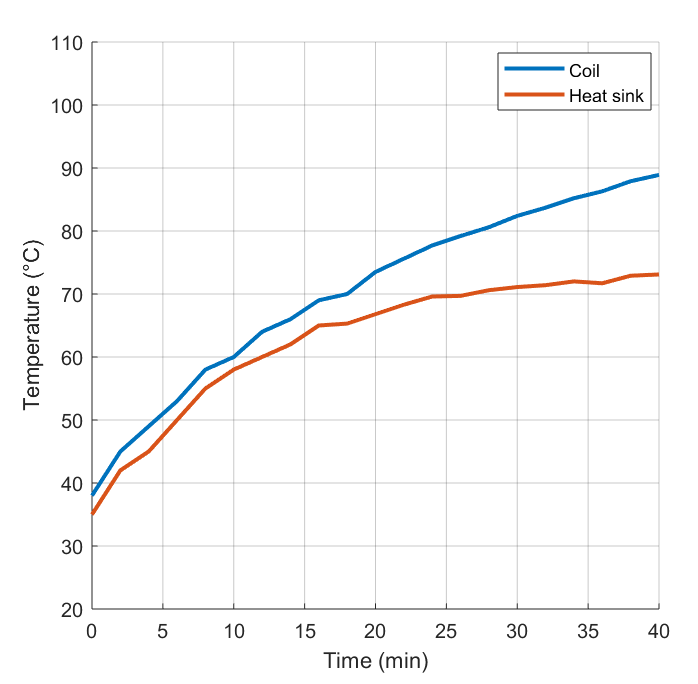
\includegraphics[width=0.65\textwidth]{../Pictures/P1/Test/Thermal_test_with_heat_sink}
		\caption{Thermal test.}
		\label{Testthermal}
	\end{center}	
\end{figure}

\subsection{MPPT test}
The MPPT test is divided into two parts as it was done for obtaining the simulation results. The test will be implemented for both modes of operation for the converter. For obtaining the results in buck mode a resistive load of 3$\Omega$ is used, and for boost mode, 27 $\Omega$.

 \subsubsection*{Standard Test Conditions (STC)}
For the first test, in both modes, the ambient condition is for irradiance 1000 $W /m^2$ and for temperature 25 $\decC$ (as STC)\todo{rephrase}. Figure \ref{MPPTtestbuckmode1} shows how the converter is tracking the MPP in buck mode. The left graph represents the input voltage and current of the converter. At first the input voltage reached the open circuit voltage as in the simulation.  After 10 seconds the P\&O algorithm reaches the MPP. The maximum average power obtained in the lab from the PV panel is 293.56 W. This can be seen in the right graph in figure \ref{MPPTtestbuckmode1}. By comparing the measured value of power with the maximum power that the PV panel can generate under these conditions, the performance of the MPPT can be quantified as shown in equation \ref{eq:effMPPTbuck}.

\begin{equation} \label{eq:effMPPTbuck}
\eta_{MPPT}= \dfrac{P_{pv}}{P_{mpp}} \cdot 100 = \dfrac{293.56W}{300.4W} \cdot 100 = 97.72\%  
\end{equation}


\begin{figure}[H]
	\begin{center}
		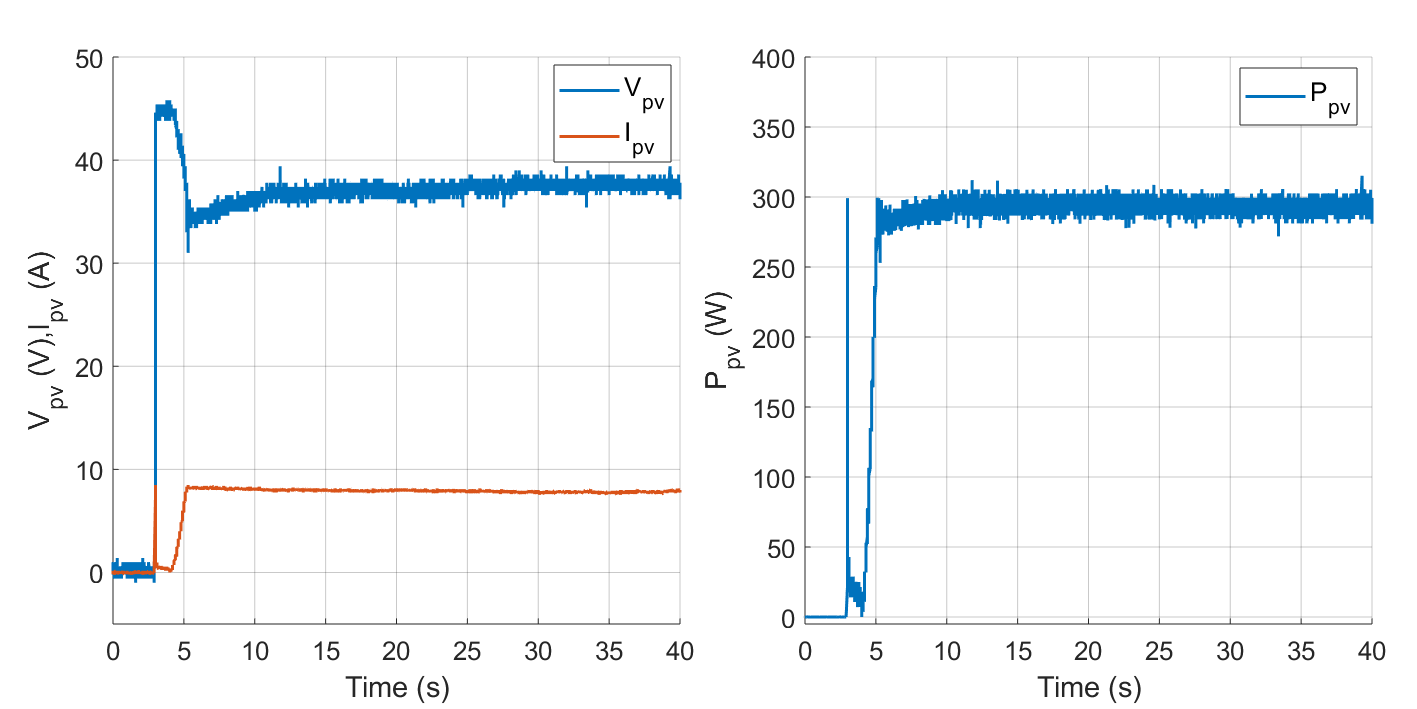
\includegraphics[width=1\textwidth]{../Pictures/P1/Test/Buck_mode_MPPT_Vin_Iin_Pin}
		\caption{Measured voltage, current and power extracted from the PV panel ($R_{L}=3\Omega$).}
		\label{MPPTtestbuckmode1}
	\end{center}	
\end{figure}

In the left graph in figure \ref{MPPTtestbuckmode2} the relationship between input and output voltage of the converter is observed. From these measurements it is possible to calculate the duty cycle in buck mode for the optimal operating point as in equation \ref{eq:measureddutybuck}. 

\begin{equation} \label{eq:measureddutybuck}
D_{buck}= \dfrac{V_{out}}{V_{pv}} = \dfrac{28.29V}{37.25} = 0.7594
\end{equation}

The right graph shows the measured input and output power of the converter. From these measurements the efficiency of the converter is calculated in equation \ref{eq:effconverterbuck}, based on the average values from the graphs.

\begin{equation} \label{eq:effconverterbuck}
\eta_{converter}= \dfrac{P_{out}}{P_{pv}} \cdot 100 = \dfrac{273.44W}{293.56W} \cdot 100 = 93.15\% 
\end{equation}


\begin{figure}[H]
	\begin{center}
		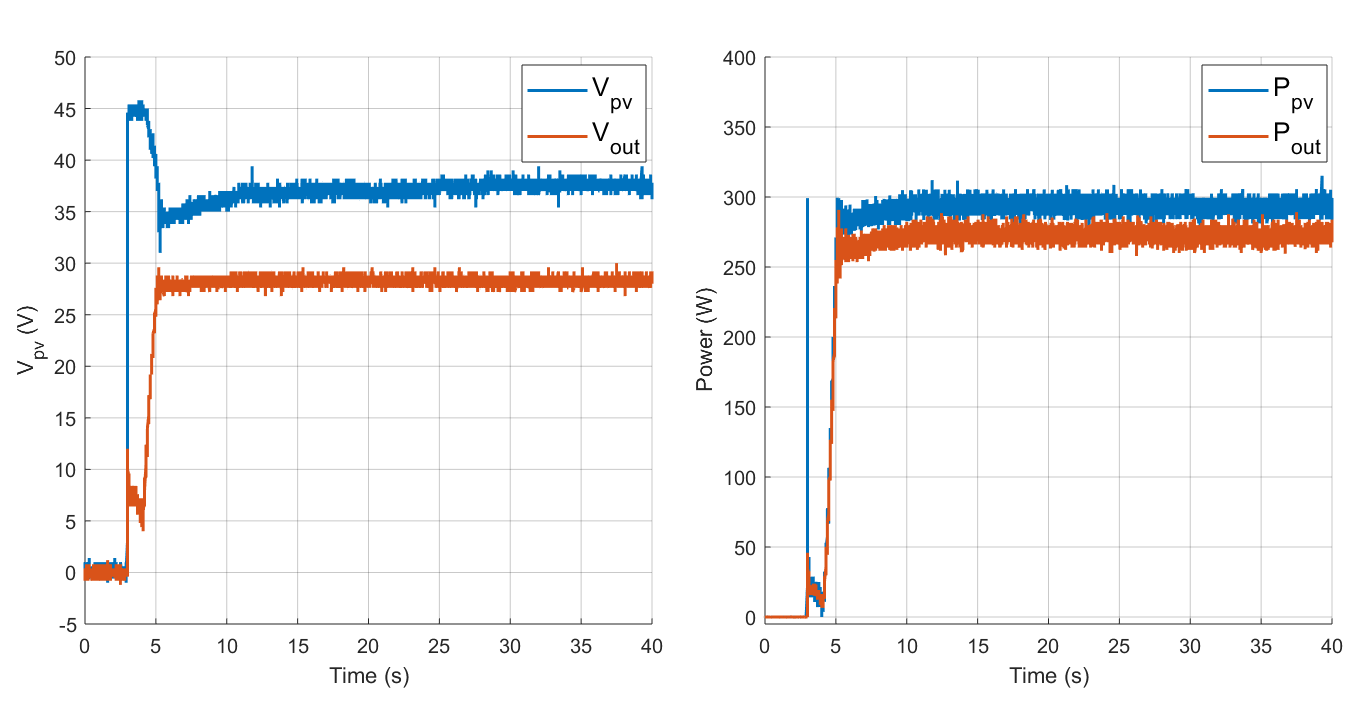
\includegraphics[width=1\textwidth]{../Pictures/P1/Test/Buck_mode_MPPT_Vin_Vout_Pin_Pout}
		\caption{Measured voltages and powers at the input and output of the converter ($R_{L}=3\Omega$).}
		\label{MPPTtestbuckmode2}
	\end{center}	
\end{figure}

Figure \ref{MPPTtestboostmode1} shows how the converter is tracking the MPP in boost mode. Here again it is observed that the MPPT is enabled after the input voltage has reached the value of open-circuit. The time the MPPT takes to reach the MPP is higher than in buck mode, reaching it in 21 seconds. By comparing the measured power with the maximum power that the PV panel can generate under STC, the MPPT's efficiency is calculated in equation \ref{eq:effMPPTboost}. It is observed that even though the system needs more time to track the MPP it does not have a significant effect in the efficiency.

\begin{equation} \label{eq:effMPPTboost}
\eta_{MPPT}= \dfrac{P_{pv}}{P_{mpp}} \cdot 100 = \dfrac{292.37W}{300.4W} \cdot 100 = 97.32\%  
\end{equation}


\begin{figure}[H]
	\begin{center}
		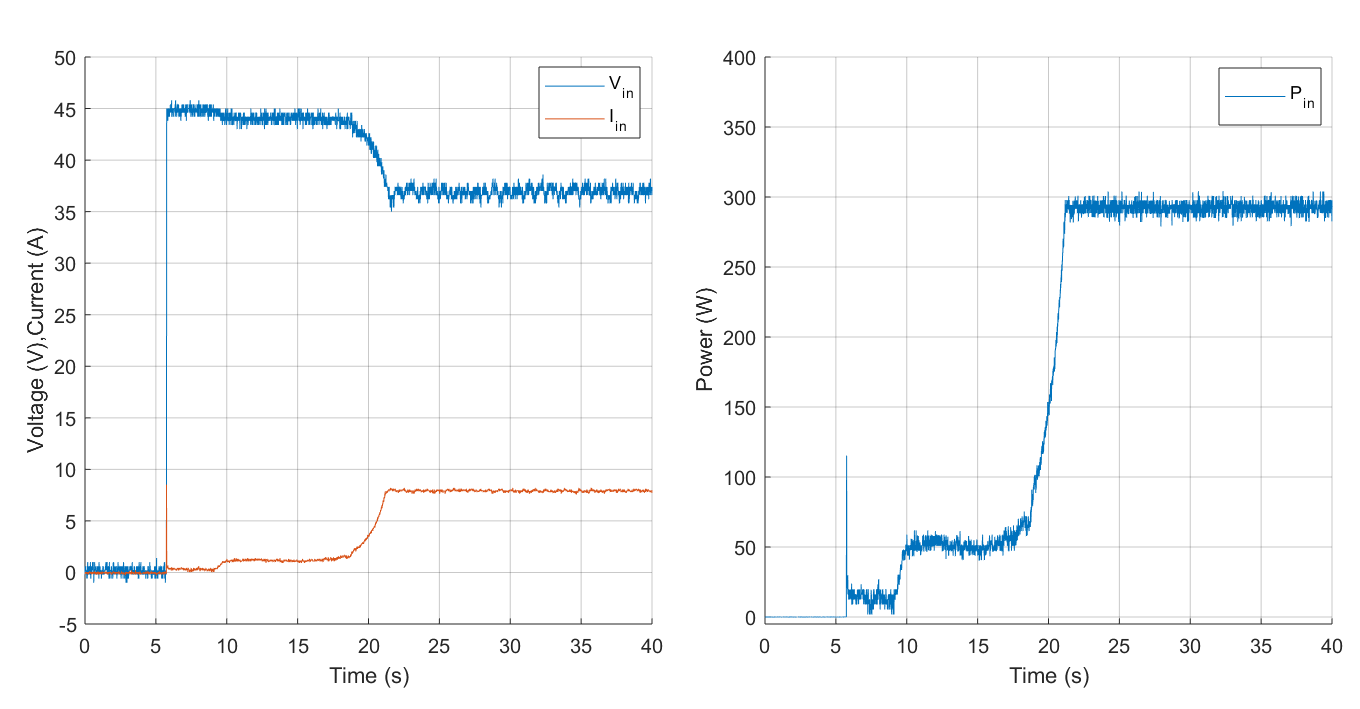
\includegraphics[width=1\textwidth]{../Pictures/P1/Test/Boost_mode_MPPT_Vin_Iin_Pin}
		\caption{Measured voltage, current and power extracted from the PV panel ($R_{L}=27\Omega$). picture not right! change axis labels and legend}
		\label{MPPTtestboostmode1}
	\end{center}	
\end{figure}

From the left graph of figure \ref{MPPTtestboostmode2} the duty cycle in boost mode for the optimal operating point can be calculated as in equation \ref{eq:measureddutyboost}. From the right graph the converter's efficiency is calculated as shown in equation \ref{eq:effconverterboost}.

\begin{equation} \label{eq:measureddutyboost}
D_{boost}= 1 - \dfrac{V_{pv}}{V_{out}} = 1 - \dfrac{36.93V}{88.41V} = 0.5823
\end{equation}

\begin{equation} \label{eq:effconverterboost}
\eta_{converter}= \dfrac{P_{out}}{P_{pv}} \cdot 100 = \dfrac{297.5W}{292.37W} \cdot 100 = 101.75\% 
\end{equation}
\todo{CHECK THIS AND DECIDE WHAT TO DO!! STEF}

\begin{figure}[H]
	\begin{center}
		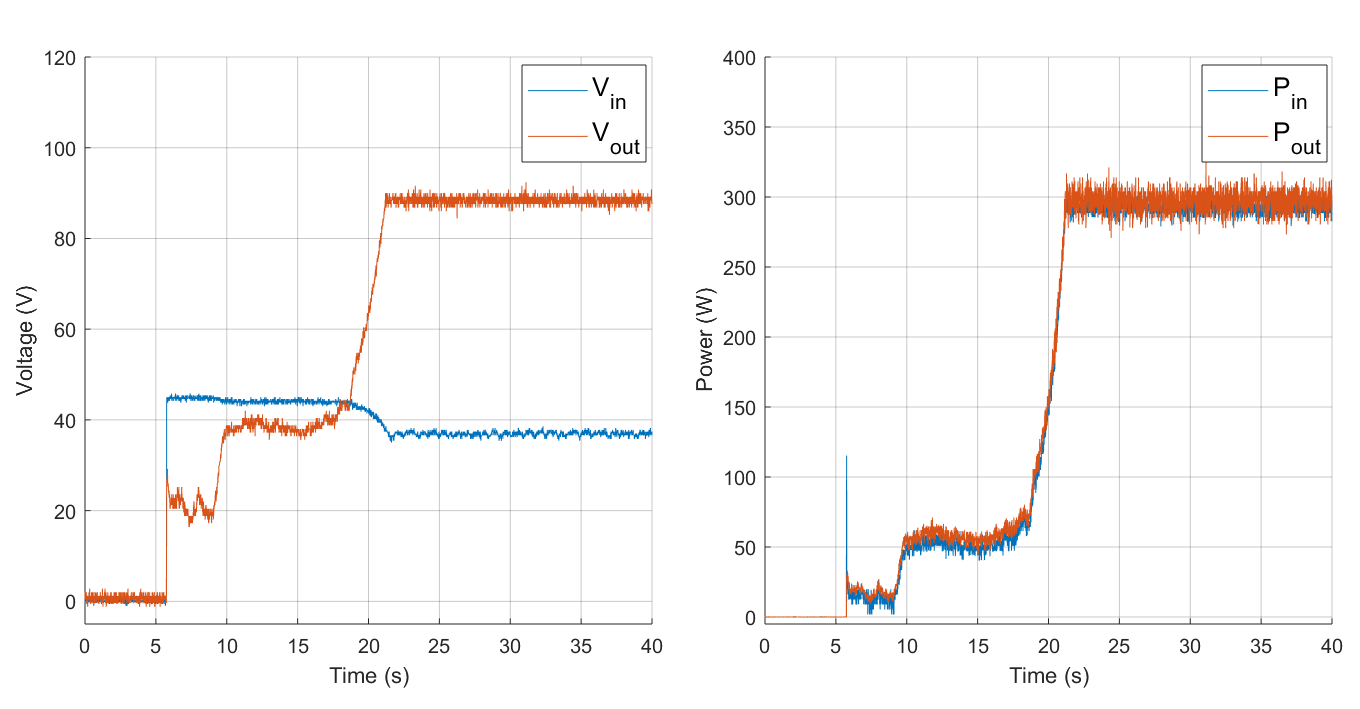
\includegraphics[width=1\textwidth]{../Pictures/P1/Test/Boost_mode_MPPT_Vin_Vout_Iin_Pin_Pout}
		\caption{Measured voltages and powers at the input and output of the converter ($R_{L}=27\Omega$).}
		\label{MPPTtestboostmode2}
	\end{center}	
\end{figure}



\subsubsection*{Change in irradiance and temperature}

For this test the converter was set to work in buck mode by fixing a resistive load of 3$\Omega$. Figure \ref{MPPTtestbuckmodeir} shows the measurements obtained for voltage, current and power generated by the PV simulator. It is observed that the MPPT detects the change in irradiance and tracks the MPP. The MPPT's efficiency changes from 95.96\% to 93.78\% when a sudden change in irradiance from 1000-800$W/m^2$ is detected. The time response is 6.6 seconds.

\begin{figure}[H]
	\begin{center}
		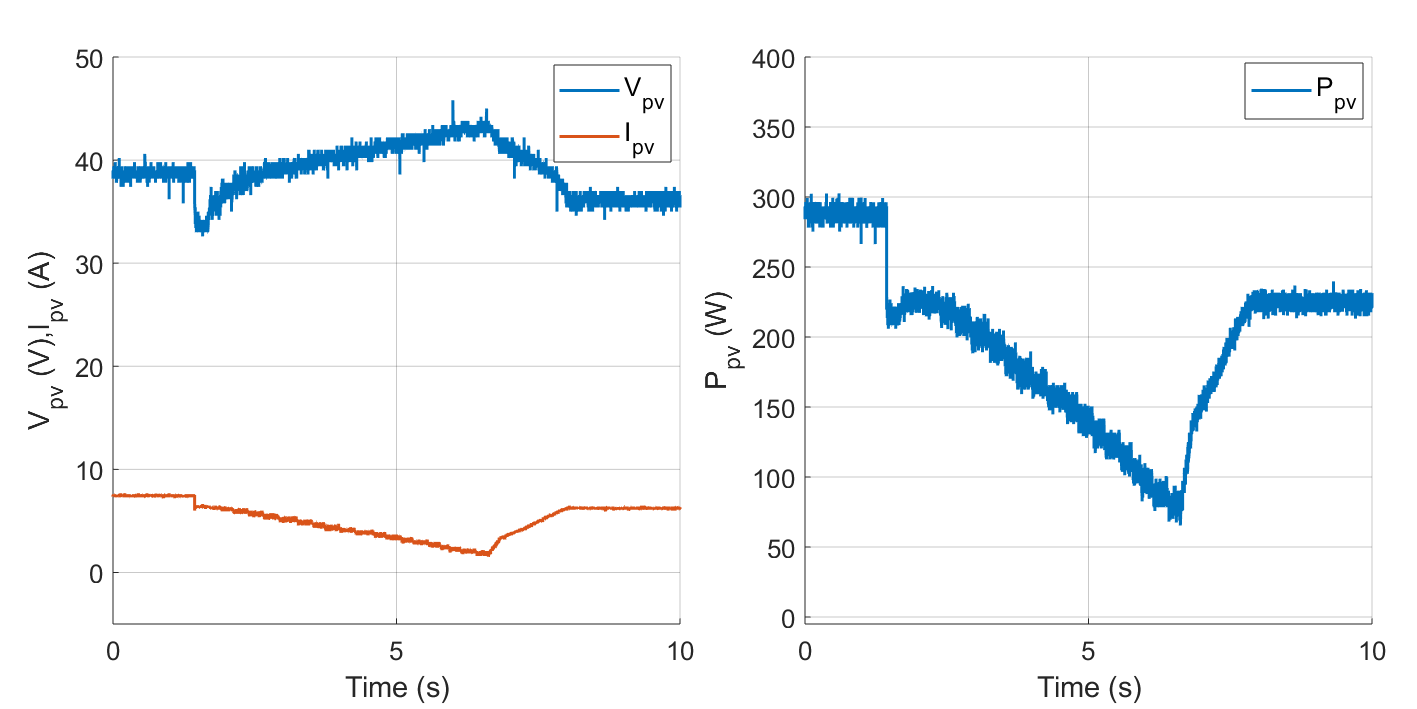
\includegraphics[width=1\textwidth]{../Pictures/P1/Test/Buck_mode_MPPT_Vin_Iin_Pin_irriadance_change}
		\caption{Measured voltage,current and powers at the input of the converter with a change in irradiance from 1000$W/m^2$ to 800$W/m^2$ ($R_{L}=3\Omega$).}
		\label{MPPTtestbuckmodeir}
	\end{center}	
\end{figure}

Figure \ref{MPPTtestbuckmodet} shows the results obtained for a sudden change in temperature from 25$\decC$ to 15$\decC$. It is observed that the generated power increases with decreasing temperature. The MPPT's efficiency improves in this case comparing with the variation in irradiance. It changes from 99.2\% to 98.4\% in 4.1 seconds. 

\begin{figure}[H]
	\begin{center}
		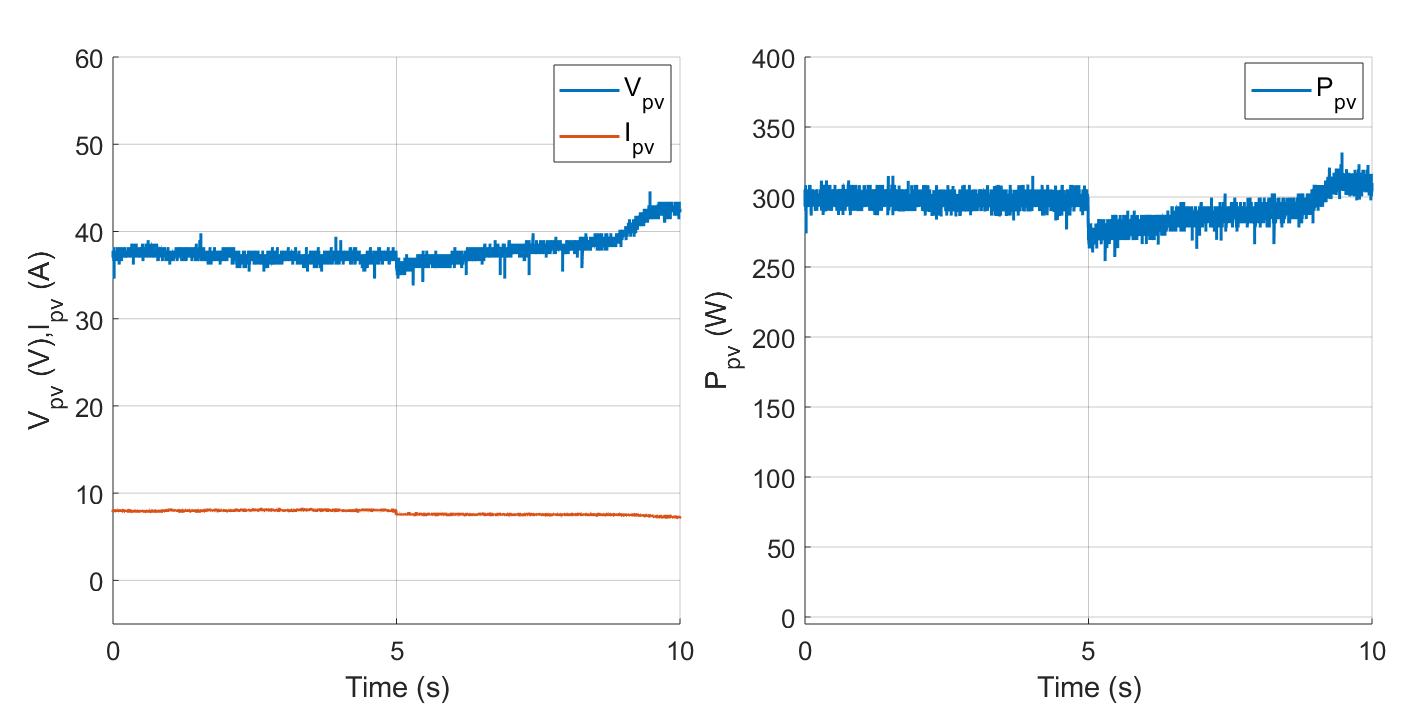
\includegraphics[width=1\textwidth]{../Pictures/P1/Test/Buck_mode_MPPT_Vin_Iin_Pin_temperature_change}
		\caption{Measured voltage,current and power at the input of the converter with a change in temperature from 25$\decC$ to 15$\decC$ ($R_{L}=3\Omega$).}
		\label{MPPTtestbuckmodet}
	\end{center}	
\end{figure}